% Options for packages loaded elsewhere
\PassOptionsToPackage{unicode}{hyperref}
\PassOptionsToPackage{hyphens}{url}
%
\documentclass[
]{article}
\usepackage{amsmath,amssymb}
\usepackage{iftex}
\ifPDFTeX
  \usepackage[T1]{fontenc}
  \usepackage[utf8]{inputenc}
  \usepackage{textcomp} % provide euro and other symbols
\else % if luatex or xetex
  \usepackage{unicode-math} % this also loads fontspec
  \defaultfontfeatures{Scale=MatchLowercase}
  \defaultfontfeatures[\rmfamily]{Ligatures=TeX,Scale=1}
\fi
\usepackage{lmodern}
\ifPDFTeX\else
  % xetex/luatex font selection
\fi
% Use upquote if available, for straight quotes in verbatim environments
\IfFileExists{upquote.sty}{\usepackage{upquote}}{}
\IfFileExists{microtype.sty}{% use microtype if available
  \usepackage[]{microtype}
  \UseMicrotypeSet[protrusion]{basicmath} % disable protrusion for tt fonts
}{}
\makeatletter
\@ifundefined{KOMAClassName}{% if non-KOMA class
  \IfFileExists{parskip.sty}{%
    \usepackage{parskip}
  }{% else
    \setlength{\parindent}{0pt}
    \setlength{\parskip}{6pt plus 2pt minus 1pt}}
}{% if KOMA class
  \KOMAoptions{parskip=half}}
\makeatother
\usepackage{xcolor}
\usepackage[margin=1in]{geometry}
\usepackage{color}
\usepackage{fancyvrb}
\newcommand{\VerbBar}{|}
\newcommand{\VERB}{\Verb[commandchars=\\\{\}]}
\DefineVerbatimEnvironment{Highlighting}{Verbatim}{commandchars=\\\{\}}
% Add ',fontsize=\small' for more characters per line
\usepackage{framed}
\definecolor{shadecolor}{RGB}{248,248,248}
\newenvironment{Shaded}{\begin{snugshade}}{\end{snugshade}}
\newcommand{\AlertTok}[1]{\textcolor[rgb]{0.94,0.16,0.16}{#1}}
\newcommand{\AnnotationTok}[1]{\textcolor[rgb]{0.56,0.35,0.01}{\textbf{\textit{#1}}}}
\newcommand{\AttributeTok}[1]{\textcolor[rgb]{0.13,0.29,0.53}{#1}}
\newcommand{\BaseNTok}[1]{\textcolor[rgb]{0.00,0.00,0.81}{#1}}
\newcommand{\BuiltInTok}[1]{#1}
\newcommand{\CharTok}[1]{\textcolor[rgb]{0.31,0.60,0.02}{#1}}
\newcommand{\CommentTok}[1]{\textcolor[rgb]{0.56,0.35,0.01}{\textit{#1}}}
\newcommand{\CommentVarTok}[1]{\textcolor[rgb]{0.56,0.35,0.01}{\textbf{\textit{#1}}}}
\newcommand{\ConstantTok}[1]{\textcolor[rgb]{0.56,0.35,0.01}{#1}}
\newcommand{\ControlFlowTok}[1]{\textcolor[rgb]{0.13,0.29,0.53}{\textbf{#1}}}
\newcommand{\DataTypeTok}[1]{\textcolor[rgb]{0.13,0.29,0.53}{#1}}
\newcommand{\DecValTok}[1]{\textcolor[rgb]{0.00,0.00,0.81}{#1}}
\newcommand{\DocumentationTok}[1]{\textcolor[rgb]{0.56,0.35,0.01}{\textbf{\textit{#1}}}}
\newcommand{\ErrorTok}[1]{\textcolor[rgb]{0.64,0.00,0.00}{\textbf{#1}}}
\newcommand{\ExtensionTok}[1]{#1}
\newcommand{\FloatTok}[1]{\textcolor[rgb]{0.00,0.00,0.81}{#1}}
\newcommand{\FunctionTok}[1]{\textcolor[rgb]{0.13,0.29,0.53}{\textbf{#1}}}
\newcommand{\ImportTok}[1]{#1}
\newcommand{\InformationTok}[1]{\textcolor[rgb]{0.56,0.35,0.01}{\textbf{\textit{#1}}}}
\newcommand{\KeywordTok}[1]{\textcolor[rgb]{0.13,0.29,0.53}{\textbf{#1}}}
\newcommand{\NormalTok}[1]{#1}
\newcommand{\OperatorTok}[1]{\textcolor[rgb]{0.81,0.36,0.00}{\textbf{#1}}}
\newcommand{\OtherTok}[1]{\textcolor[rgb]{0.56,0.35,0.01}{#1}}
\newcommand{\PreprocessorTok}[1]{\textcolor[rgb]{0.56,0.35,0.01}{\textit{#1}}}
\newcommand{\RegionMarkerTok}[1]{#1}
\newcommand{\SpecialCharTok}[1]{\textcolor[rgb]{0.81,0.36,0.00}{\textbf{#1}}}
\newcommand{\SpecialStringTok}[1]{\textcolor[rgb]{0.31,0.60,0.02}{#1}}
\newcommand{\StringTok}[1]{\textcolor[rgb]{0.31,0.60,0.02}{#1}}
\newcommand{\VariableTok}[1]{\textcolor[rgb]{0.00,0.00,0.00}{#1}}
\newcommand{\VerbatimStringTok}[1]{\textcolor[rgb]{0.31,0.60,0.02}{#1}}
\newcommand{\WarningTok}[1]{\textcolor[rgb]{0.56,0.35,0.01}{\textbf{\textit{#1}}}}
\usepackage{graphicx}
\makeatletter
\def\maxwidth{\ifdim\Gin@nat@width>\linewidth\linewidth\else\Gin@nat@width\fi}
\def\maxheight{\ifdim\Gin@nat@height>\textheight\textheight\else\Gin@nat@height\fi}
\makeatother
% Scale images if necessary, so that they will not overflow the page
% margins by default, and it is still possible to overwrite the defaults
% using explicit options in \includegraphics[width, height, ...]{}
\setkeys{Gin}{width=\maxwidth,height=\maxheight,keepaspectratio}
% Set default figure placement to htbp
\makeatletter
\def\fps@figure{htbp}
\makeatother
\setlength{\emergencystretch}{3em} % prevent overfull lines
\providecommand{\tightlist}{%
  \setlength{\itemsep}{0pt}\setlength{\parskip}{0pt}}
\setcounter{secnumdepth}{-\maxdimen} % remove section numbering
\ifLuaTeX
  \usepackage{selnolig}  % disable illegal ligatures
\fi
\IfFileExists{bookmark.sty}{\usepackage{bookmark}}{\usepackage{hyperref}}
\IfFileExists{xurl.sty}{\usepackage{xurl}}{} % add URL line breaks if available
\urlstyle{same}
\hypersetup{
  pdftitle={Relationship between User Reviews and Critic Reviews},
  pdfauthor={Zihan Ma},
  hidelinks,
  pdfcreator={LaTeX via pandoc}}

\title{Relationship between User Reviews and Critic Reviews}
\author{Zihan Ma}
\date{2023-08-10}

\begin{document}
\maketitle

\hypertarget{scatterplot-of-user-reviews-vs-critic-reviews}{%
\subsection{Scatterplot of User Reviews vs Critic
Reviews}\label{scatterplot-of-user-reviews-vs-critic-reviews}}

\begin{Shaded}
\begin{Highlighting}[]
\CommentTok{\# Load necessary libraries}
\FunctionTok{library}\NormalTok{(readr)}
\FunctionTok{library}\NormalTok{(ggplot2)}
\FunctionTok{library}\NormalTok{(dplyr)}
\FunctionTok{library}\NormalTok{(tidyr)}
\CommentTok{\# library(visdat)}
\FunctionTok{library}\NormalTok{(rpart)}
\FunctionTok{library}\NormalTok{(rpart.plot,}\AttributeTok{quietly =} \ConstantTok{TRUE}\NormalTok{)}
\end{Highlighting}
\end{Shaded}

\begin{Shaded}
\begin{Highlighting}[]
\NormalTok{Oscar\_2000\_2018 }\OtherTok{\textless{}{-}} \FunctionTok{read\_csv}\NormalTok{(}\StringTok{"DataSets/Oscar\_2000\_2018.csv"}\NormalTok{)}
\end{Highlighting}
\end{Shaded}

\begin{verbatim}
## Rows: 1235 Columns: 119
## -- Column specification --------------------------------------------------------
## Delimiter: ","
## chr  (62): movie, movie_id, certificate, genre, synopsis, Oscar_Best_Picture...
## dbl  (56): year, duration, rate, metascore, votes, gross, user_reviews, crit...
## date  (1): release_date
## 
## i Use `spec()` to retrieve the full column specification for this data.
## i Specify the column types or set `show_col_types = FALSE` to quiet this message.
\end{verbatim}

\begin{Shaded}
\begin{Highlighting}[]
\CommentTok{\# View(Oscar\_2000\_2018)}
\end{Highlighting}
\end{Shaded}

\begin{Shaded}
\begin{Highlighting}[]
\CommentTok{\# Calculate the percentage of missing values for user\_reviews}
\NormalTok{percent\_missing\_user\_reviews }\OtherTok{\textless{}{-}} \FunctionTok{sum}\NormalTok{(}\FunctionTok{is.na}\NormalTok{(Oscar\_2000\_2018}\SpecialCharTok{$}\NormalTok{user\_reviews)) }\SpecialCharTok{/} \FunctionTok{nrow}\NormalTok{(Oscar\_2000\_2018) }\SpecialCharTok{*} \DecValTok{100}

\CommentTok{\# Calculate the percentage of missing values for critic\_reviews}
\NormalTok{percent\_missing\_critic\_reviews }\OtherTok{\textless{}{-}} \FunctionTok{sum}\NormalTok{(}\FunctionTok{is.na}\NormalTok{(Oscar\_2000\_2018}\SpecialCharTok{$}\NormalTok{critic\_reviews)) }\SpecialCharTok{/} \FunctionTok{nrow}\NormalTok{(Oscar\_2000\_2018) }\SpecialCharTok{*} \DecValTok{100}

\NormalTok{percent\_missing\_user\_reviews}
\end{Highlighting}
\end{Shaded}

\begin{verbatim}
## [1] 1.133603
\end{verbatim}

\begin{Shaded}
\begin{Highlighting}[]
\NormalTok{percent\_missing\_critic\_reviews}
\end{Highlighting}
\end{Shaded}

\begin{verbatim}
## [1] 0.8097166
\end{verbatim}

\begin{Shaded}
\begin{Highlighting}[]
\CommentTok{\# Remove rows with missing values in user\_reviews and critic\_reviews columns}
\NormalTok{Oscar\_2000\_2018\_cleaned }\OtherTok{\textless{}{-}}\NormalTok{ Oscar\_2000\_2018[}\SpecialCharTok{!}\FunctionTok{is.na}\NormalTok{(Oscar\_2000\_2018}\SpecialCharTok{$}\NormalTok{user\_reviews) }\SpecialCharTok{\&} \SpecialCharTok{!}\FunctionTok{is.na}\NormalTok{(Oscar\_2000\_2018}\SpecialCharTok{$}\NormalTok{critic\_reviews), ]}
\end{Highlighting}
\end{Shaded}

\begin{Shaded}
\begin{Highlighting}[]
\CommentTok{\# Plotting the scatterplot}
\FunctionTok{ggplot}\NormalTok{(Oscar\_2000\_2018\_cleaned, }\FunctionTok{aes}\NormalTok{(}\AttributeTok{x=}\NormalTok{user\_reviews, }\AttributeTok{y=}\NormalTok{critic\_reviews)) }\SpecialCharTok{+}
  \FunctionTok{geom\_point}\NormalTok{(}\AttributeTok{alpha=}\FloatTok{0.5}\NormalTok{) }\SpecialCharTok{+}
  \FunctionTok{ggtitle}\NormalTok{(}\StringTok{"Scatterplot of User Reviews vs Critic Reviews"}\NormalTok{) }\SpecialCharTok{+}
  \FunctionTok{xlab}\NormalTok{(}\StringTok{"User Reviews"}\NormalTok{) }\SpecialCharTok{+}
  \FunctionTok{ylab}\NormalTok{(}\StringTok{"Critic Reviews"}\NormalTok{)}
\end{Highlighting}
\end{Shaded}

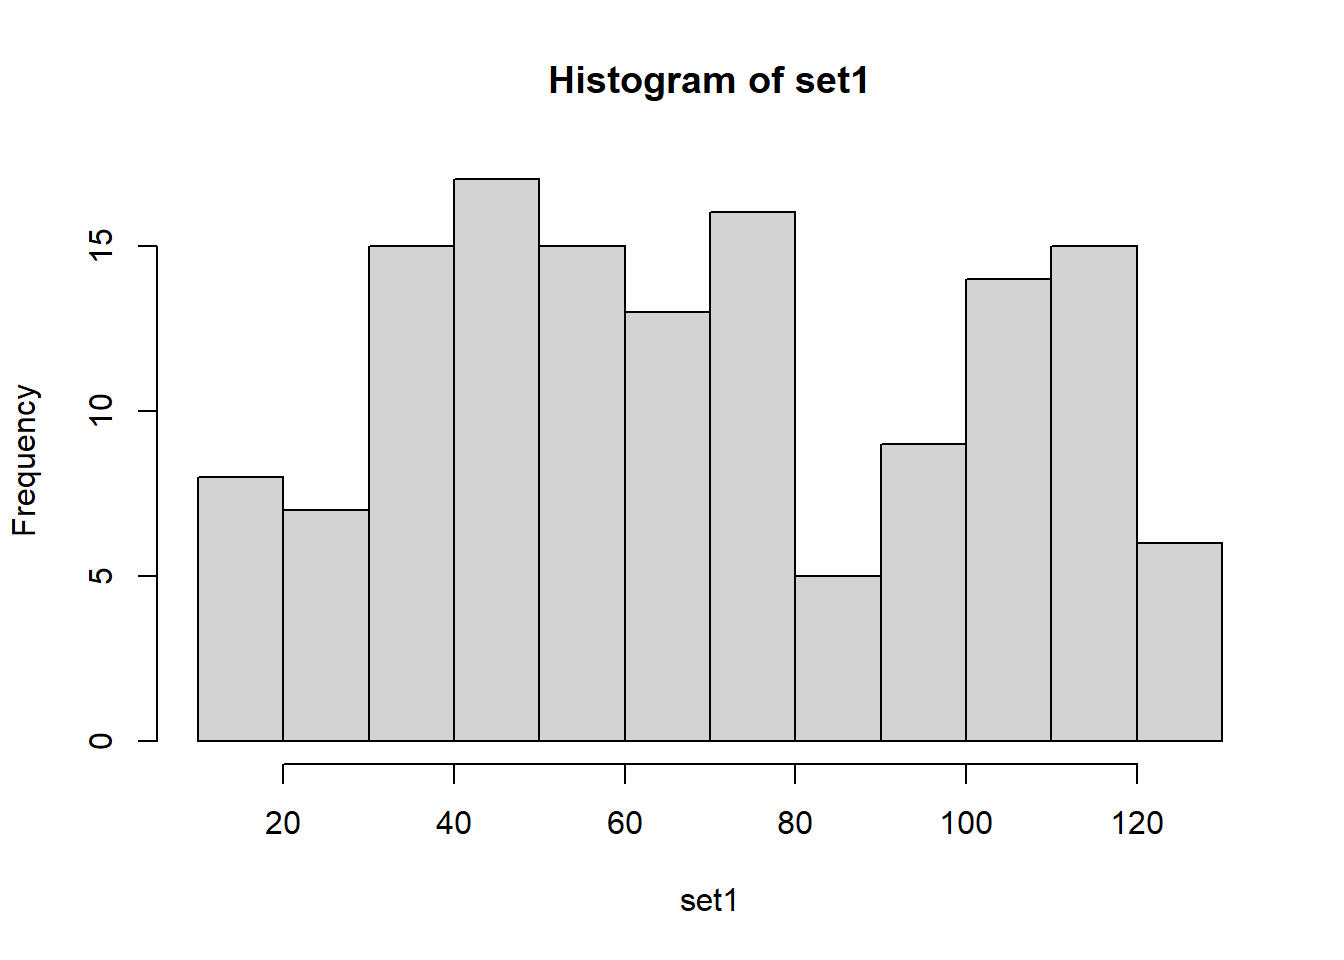
\includegraphics{Week5-IndivudualQuiz_files/figure-latex/unnamed-chunk-5-1.pdf}

\begin{Shaded}
\begin{Highlighting}[]
\CommentTok{\# Calculate Pearson\textquotesingle{}s correlation coefficient}
\NormalTok{correlation\_coefficient\_cleaned }\OtherTok{\textless{}{-}} \FunctionTok{cor}\NormalTok{(Oscar\_2000\_2018\_cleaned}\SpecialCharTok{$}\NormalTok{user\_reviews, Oscar\_2000\_2018\_cleaned}\SpecialCharTok{$}\NormalTok{critic\_reviews)}
\NormalTok{correlation\_coefficient\_cleaned}
\end{Highlighting}
\end{Shaded}

\begin{verbatim}
## [1] 0.4958438
\end{verbatim}

\begin{Shaded}
\begin{Highlighting}[]
\CommentTok{\# Group by certificate and calculate average duration}
\NormalTok{avg\_duration\_per\_certificate }\OtherTok{\textless{}{-}}\NormalTok{ Oscar\_2000\_2018 }\SpecialCharTok{\%\textgreater{}\%}
  \FunctionTok{group\_by}\NormalTok{(certificate) }\SpecialCharTok{\%\textgreater{}\%}
  \FunctionTok{summarise}\NormalTok{(}\AttributeTok{avg\_duration =} \FunctionTok{mean}\NormalTok{(duration, }\AttributeTok{na.rm =} \ConstantTok{TRUE}\NormalTok{))}
\end{Highlighting}
\end{Shaded}

\begin{Shaded}
\begin{Highlighting}[]
\CommentTok{\# Plotting}
\FunctionTok{ggplot}\NormalTok{(avg\_duration\_per\_certificate, }\FunctionTok{aes}\NormalTok{(}\AttributeTok{x=}\NormalTok{certificate, }\AttributeTok{y=}\NormalTok{avg\_duration)) }\SpecialCharTok{+}
  \FunctionTok{geom\_bar}\NormalTok{(}\AttributeTok{stat=}\StringTok{"identity"}\NormalTok{, }\AttributeTok{fill=}\StringTok{"steelblue"}\NormalTok{) }\SpecialCharTok{+}
  \FunctionTok{ggtitle}\NormalTok{(}\StringTok{"Average Duration per Certificate"}\NormalTok{) }\SpecialCharTok{+}
  \FunctionTok{xlab}\NormalTok{(}\StringTok{"Certificate"}\NormalTok{) }\SpecialCharTok{+}
  \FunctionTok{ylab}\NormalTok{(}\StringTok{"Average Duration"}\NormalTok{) }\SpecialCharTok{+}
  \FunctionTok{theme\_minimal}\NormalTok{() }\SpecialCharTok{+}
  \FunctionTok{theme}\NormalTok{(}\AttributeTok{axis.text.x =} \FunctionTok{element\_text}\NormalTok{(}\AttributeTok{angle =} \DecValTok{45}\NormalTok{, }\AttributeTok{hjust =} \DecValTok{1}\NormalTok{))}
\end{Highlighting}
\end{Shaded}

\includegraphics{Week5-IndivudualQuiz_files/figure-latex/unnamed-chunk-8-1.pdf}

\begin{Shaded}
\begin{Highlighting}[]
\CommentTok{\# Split the genre column and gather them into a single column}
\NormalTok{split\_genres }\OtherTok{\textless{}{-}}\NormalTok{ Oscar\_2000\_2018 }\SpecialCharTok{\%\textgreater{}\%}
  \FunctionTok{mutate}\NormalTok{(}\AttributeTok{genre =} \FunctionTok{strsplit}\NormalTok{(}\FunctionTok{as.character}\NormalTok{(genre), }\StringTok{"}\SpecialCharTok{\textbackslash{}\textbackslash{}}\StringTok{|"}\NormalTok{)) }\SpecialCharTok{\%\textgreater{}\%}
  \FunctionTok{unnest}\NormalTok{(genre)}

\CommentTok{\# Count the frequency of each genre}
\NormalTok{genre\_counts }\OtherTok{\textless{}{-}}\NormalTok{ split\_genres }\SpecialCharTok{\%\textgreater{}\%}
  \FunctionTok{group\_by}\NormalTok{(genre) }\SpecialCharTok{\%\textgreater{}\%}
  \FunctionTok{tally}\NormalTok{() }\SpecialCharTok{\%\textgreater{}\%}
  \FunctionTok{arrange}\NormalTok{(}\SpecialCharTok{{-}}\NormalTok{n)}

\CommentTok{\# Plotting the histogram}
\FunctionTok{ggplot}\NormalTok{(genre\_counts, }\FunctionTok{aes}\NormalTok{(}\AttributeTok{x=}\FunctionTok{reorder}\NormalTok{(genre, n), }\AttributeTok{y=}\NormalTok{n)) }\SpecialCharTok{+}
  \FunctionTok{geom\_bar}\NormalTok{(}\AttributeTok{stat=}\StringTok{"identity"}\NormalTok{, }\AttributeTok{fill=}\StringTok{"steelblue"}\NormalTok{) }\SpecialCharTok{+}
  \FunctionTok{coord\_flip}\NormalTok{() }\SpecialCharTok{+}
  \FunctionTok{ggtitle}\NormalTok{(}\StringTok{"Frequency of Each Genre"}\NormalTok{) }\SpecialCharTok{+}
  \FunctionTok{xlab}\NormalTok{(}\StringTok{"Genre"}\NormalTok{) }\SpecialCharTok{+}
  \FunctionTok{ylab}\NormalTok{(}\StringTok{"Frequency"}\NormalTok{) }\SpecialCharTok{+}
  \FunctionTok{theme\_minimal}\NormalTok{()}
\end{Highlighting}
\end{Shaded}

\includegraphics{Week5-IndivudualQuiz_files/figure-latex/unnamed-chunk-9-1.pdf}

\begin{Shaded}
\begin{Highlighting}[]
\CommentTok{\# Removing columns with convention "Oscar\_Best\_XXX\_won" except for "Oscar\_Best\_Picture\_won"}
\NormalTok{cols\_to\_remove }\OtherTok{\textless{}{-}} \FunctionTok{grep}\NormalTok{(}\StringTok{"\^{}Oscar\_Best\_.*\_won$"}\NormalTok{, }\FunctionTok{names}\NormalTok{(Oscar\_2000\_2018), }\AttributeTok{value =} \ConstantTok{TRUE}\NormalTok{)}
\NormalTok{cols\_to\_remove }\OtherTok{\textless{}{-}} \FunctionTok{setdiff}\NormalTok{(cols\_to\_remove, }\StringTok{"Oscar\_Best\_Picture\_won"}\NormalTok{)}
\NormalTok{Oscar\_2000\_2018 }\OtherTok{\textless{}{-}}\NormalTok{ Oscar\_2000\_2018[, }\SpecialCharTok{!}\FunctionTok{names}\NormalTok{(Oscar\_2000\_2018) }\SpecialCharTok{\%in\%}\NormalTok{ cols\_to\_remove]}
\end{Highlighting}
\end{Shaded}

\begin{Shaded}
\begin{Highlighting}[]
\CommentTok{\# Convert target variable to numerical type}
\NormalTok{Oscar\_2000\_2018}\SpecialCharTok{$}\NormalTok{Oscar\_Best\_Picture\_won }\OtherTok{\textless{}{-}} \FunctionTok{ifelse}\NormalTok{(Oscar\_2000\_2018}\SpecialCharTok{$}\NormalTok{Oscar\_Best\_Picture\_won }\SpecialCharTok{==} \StringTok{"Yes"}\NormalTok{, }\DecValTok{1}\NormalTok{, }\DecValTok{0}\NormalTok{)}
\end{Highlighting}
\end{Shaded}

\begin{Shaded}
\begin{Highlighting}[]
\CommentTok{\# Identify columns with over 70\% NAs}
\NormalTok{cols\_with\_nas }\OtherTok{\textless{}{-}} \FunctionTok{names}\NormalTok{(Oscar\_2000\_2018)[}\FunctionTok{sapply}\NormalTok{(Oscar\_2000\_2018, }\ControlFlowTok{function}\NormalTok{(col) \{}
  \FunctionTok{mean}\NormalTok{(}\FunctionTok{is.na}\NormalTok{(col)) }\SpecialCharTok{\textgreater{}} \FloatTok{0.7}
\NormalTok{\})]}

\CommentTok{\# Combine with high cardinality columns removal, if you want}
\CommentTok{\# Identify columns with high cardinality}
\NormalTok{threshold }\OtherTok{\textless{}{-}} \FloatTok{0.05} \SpecialCharTok{*} \FunctionTok{nrow}\NormalTok{(Oscar\_2000\_2018)}
\NormalTok{cols\_high\_cardinality }\OtherTok{\textless{}{-}} \FunctionTok{names}\NormalTok{(Oscar\_2000\_2018)[}\FunctionTok{sapply}\NormalTok{(Oscar\_2000\_2018, }\ControlFlowTok{function}\NormalTok{(col) \{}
  \FunctionTok{length}\NormalTok{(}\FunctionTok{unique}\NormalTok{(col)) }\SpecialCharTok{\textgreater{}}\NormalTok{ threshold}
\NormalTok{\})]}

\CommentTok{\# Merge the two lists of columns to remove}
\NormalTok{cols\_to\_remove }\OtherTok{\textless{}{-}} \FunctionTok{unique}\NormalTok{(}\FunctionTok{c}\NormalTok{(cols\_with\_nas, cols\_high\_cardinality))}

\CommentTok{\# Remove those columns from the dataset}
\NormalTok{Oscar\_2000\_2018 }\OtherTok{\textless{}{-}}\NormalTok{ Oscar\_2000\_2018[, }\SpecialCharTok{!}\FunctionTok{names}\NormalTok{(Oscar\_2000\_2018) }\SpecialCharTok{\%in\%}\NormalTok{ cols\_to\_remove]}
\end{Highlighting}
\end{Shaded}

\begin{Shaded}
\begin{Highlighting}[]
\CommentTok{\# Splitting data based on year for training and testing}
\NormalTok{train\_data }\OtherTok{\textless{}{-}}\NormalTok{ Oscar\_2000\_2018[Oscar\_2000\_2018}\SpecialCharTok{$}\NormalTok{year }\SpecialCharTok{\textless{}=} \DecValTok{2017}\NormalTok{, ]}
\NormalTok{test\_data }\OtherTok{\textless{}{-}}\NormalTok{ Oscar\_2000\_2018[Oscar\_2000\_2018}\SpecialCharTok{$}\NormalTok{year }\SpecialCharTok{==} \DecValTok{2018}\NormalTok{, ]}
\NormalTok{test\_data}\SpecialCharTok{$}\NormalTok{certificate[test\_data}\SpecialCharTok{$}\NormalTok{certificate }\SpecialCharTok{==} \StringTok{"TV{-}PG"}\NormalTok{] }\OtherTok{\textless{}{-}} \StringTok{"PG"}
\end{Highlighting}
\end{Shaded}

\begin{Shaded}
\begin{Highlighting}[]
\NormalTok{tree\_model }\OtherTok{\textless{}{-}} \FunctionTok{rpart}\NormalTok{(Oscar\_Best\_Picture\_won }\SpecialCharTok{\textasciitilde{}}\NormalTok{ rate }\SpecialCharTok{+}\NormalTok{ awards\_wins }\SpecialCharTok{+}\NormalTok{ Golden\_Globes\_won, }\AttributeTok{data=}\NormalTok{train\_data)}
\FunctionTok{summary}\NormalTok{(tree\_model)}
\end{Highlighting}
\end{Shaded}

\begin{verbatim}
## Call:
## rpart(formula = Oscar_Best_Picture_won ~ rate + awards_wins + 
##     Golden_Globes_won, data = train_data)
##   n= 1183 
## 
##           CP nsplit rel error    xerror      xstd
## 1 0.24408610      0 1.0000000 1.0012950 0.2305716
## 2 0.05976529      1 0.7559139 0.9482885 0.1871934
## 3 0.05626739      2 0.6961486 0.9201485 0.1778086
## 4 0.01485802      3 0.6398812 0.8972952 0.1651293
## 5 0.01000000      4 0.6250232 0.8780709 0.1623439
## 
## Variable importance
##       awards_wins Golden_Globes_won              rate 
##                76                16                 8 
## 
## Node number 1: 1183 observations,    complexity param=0.2440861
##   mean=0.01521555, MSE=0.01498404 
##   left son=2 (1161 obs) right son=3 (22 obs)
##   Primary splits:
##       awards_wins       < 25.5 to the left,  improve=0.24408610, (0 missing)
##       Golden_Globes_won < 1.5  to the left,  improve=0.11826430, (0 missing)
##       rate              < 7.95 to the left,  improve=0.05043795, (0 missing)
##   Surrogate splits:
##       Golden_Globes_won < 3.5  to the left,  agree=0.984, adj=0.136, (0 split)
##       rate              < 8.75 to the left,  agree=0.983, adj=0.091, (0 split)
## 
## Node number 2: 1161 observations,    complexity param=0.05976529
##   mean=0.006890612, MSE=0.006843131 
##   left son=4 (1117 obs) right son=5 (44 obs)
##   Primary splits:
##       awards_wins       < 14.5 to the left,  improve=0.13334470, (0 missing)
##       Golden_Globes_won < 1.5  to the left,  improve=0.07273917, (0 missing)
##       rate              < 8.05 to the left,  improve=0.03248562, (0 missing)
##   Surrogate splits:
##       Golden_Globes_won < 2.5  to the left,  agree=0.972, adj=0.250, (0 split)
##       rate              < 8.65 to the left,  agree=0.964, adj=0.045, (0 split)
## 
## Node number 3: 22 observations,    complexity param=0.05626739
##   mean=0.4545455, MSE=0.2479339 
##   left son=6 (7 obs) right son=7 (15 obs)
##   Primary splits:
##       awards_wins       < 38   to the right, improve=0.18285710, (0 missing)
##       rate              < 7.95 to the left,  improve=0.04102564, (0 missing)
##       Golden_Globes_won < 1.5  to the left,  improve=0.01000000, (0 missing)
##   Surrogate splits:
##       Golden_Globes_won < 2.5  to the right, agree=0.818, adj=0.429, (0 split)
## 
## Node number 4: 1117 observations
##   mean=0.0008952551, MSE=0.0008944537 
## 
## Node number 5: 44 observations,    complexity param=0.01485802
##   mean=0.1590909, MSE=0.133781 
##   left son=10 (29 obs) right son=11 (15 obs)
##   Primary splits:
##       rate              < 8.05 to the left,  improve=0.04474327, (0 missing)
##       awards_wins       < 19.5 to the right, improve=0.03985108, (0 missing)
##       Golden_Globes_won < 1.5  to the left,  improve=0.01042471, (0 missing)
##   Surrogate splits:
##       awards_wins       < 24.5 to the left,  agree=0.727, adj=0.200, (0 split)
##       Golden_Globes_won < 3.5  to the left,  agree=0.705, adj=0.133, (0 split)
## 
## Node number 6: 7 observations
##   mean=0.1428571, MSE=0.122449 
## 
## Node number 7: 15 observations
##   mean=0.6, MSE=0.24 
## 
## Node number 10: 29 observations
##   mean=0.1034483, MSE=0.09274673 
## 
## Node number 11: 15 observations
##   mean=0.2666667, MSE=0.1955556
\end{verbatim}

\begin{Shaded}
\begin{Highlighting}[]
\CommentTok{\# Visualize the decision tree with rpart.plot}
\FunctionTok{rpart.plot}\NormalTok{(tree\_model, }\AttributeTok{nn=}\ConstantTok{TRUE}\NormalTok{)}
\end{Highlighting}
\end{Shaded}

\includegraphics{Week5-IndivudualQuiz_files/figure-latex/unnamed-chunk-15-1.pdf}

\begin{Shaded}
\begin{Highlighting}[]
\CommentTok{\# \# Predict on the test data}
\CommentTok{\# predictions \textless{}{-} predict(tree\_model, test\_data[, !names(test\_data) \%in\% "movie"], type="prob")[,2]  \# Selecting the probability of class 1 (Yes)}
\end{Highlighting}
\end{Shaded}

\hypertarget{r-find-the-movie-in-2018-associated-with-the-maximum-predicted-value-most_likely_winner---test_datamoviewhich.maxpredictions-most_likely_winner---}{%
\section{\texorpdfstring{\texttt{\{r\}\ \#\ \#\ Find\ the\ movie\ in\ 2018\ associated\ with\ the\ maximum\ predicted\ value\ \#\ most\_likely\_winner\ \textless{}-\ test\_data\$movie{[}which.max(predictions){]}\ \#\ most\_likely\_winner\ \textless{}!-\/-}
--\textgreater{}}{\{r\} \# \# Find the movie in 2018 associated with the maximum predicted value \# most\_likely\_winner \textless- test\_data\$movie{[}which.max(predictions){]} \# most\_likely\_winner \textless!-\/- --\textgreater{}}}\label{r-find-the-movie-in-2018-associated-with-the-maximum-predicted-value-most_likely_winner---test_datamoviewhich.maxpredictions-most_likely_winner---}}

\end{document}
